%auto-ignore
\documentclass[./Main-revtex.tex]{subfiles}

%%%%%%
%% no preamble in this file: subfiles uses the main file's preamble
%% --> so make sure you add your definitions there
%%%%%%

\begin{document}

\ifSubfilesClassLoaded{% then branch
    % commands executed only if this file is compiled by itself
    \title{Experimental methods}
    \date{\today}
    \maketitle
}{% else branch
    % commands executed only if compiled from the main file
}

\renewcommand{\figurename}{Extended Data FIG.}\setcounter{figure}{0}
\renewcommand{\tablename}{Extended Data TABLE}\setcounter{table}{0}

% \section{Optomechanical device}
% We monitor the motion of a high-quality mechanical resonator via optical read-out. To do so, 
% We employ an on-chip optomechanical device, consisting of a silicon nitride string coupled to a photonic crystal cavity, as shown in Fig.~1 and described in~\cite{guo2022integrated}.
% Acoustic clamping losses are minimised by a hierarchical, fractal-like clamping structure, while pre-stressing the silicon nitride reduces mechanical losses through dissipation dilution.
% Vertical integration of the optical cavity then allows strong optomechanical coupling to the fundamental out-of-plane resonance of the string, for which dissipation dilution is most effective. 
% Stiffening tethers shift the mechanical modes of the cavity structure itself to higher frequencies. 
% The device is characterised in section~\ref{sec:methods:characterisation}.

% As characterised in section~\ref{sec:methods:characterisation}, the fundamental mechanical mode resonates at $\Omega/(2\pi) = 1.04$~MHz, with intrinsic decay rate $\Gamma/(2\pi)=11.5$~mHz at cryogenic temperatures (quality factor $\mathcal{Q}=9.1 \times 10^7$). 
% The optical cavity has resonance frequency 
% $\omgc/(2\pi) = 194.898$~THz                    % full value: 194.89786 THz
% (vacuum wavelength $\lambda_0 = 1538.20$~nm)  % full value: 1538.2029 nm
% and linewidth $\kappa/(2\pi) = 11.50$~GHz, and interacts dispersively with resonator displacement at a vacuum optomechanical coupling rate $g_0/(2\pi) = 158.8$~kHz.

% The silicon nitride photonic crystal cavity is evanescently coupled to an adjacent waveguide. This waveguide is capped off at one end by a photonic crystal mirror and, at the other end, by a tapered section. By bringing the tapered section in contact with a tapered fibre, light can be coupled into and out of the cavity efficiently, as discussed in section~\ref{sec:methods:optical_coupling}. 

% \temp{Actual dimensions of the device.}
% The optomechanical device, along with several spares, is fabricated on a chip. Further details on design and fabrication can be found in~\cite{guo2022integrated}.

%(Fab details? Maybe not, not new. Can just refer to Guo 2022)
%SOI process, EBL, RIE, isotropic HF wet etch. Vertical assembly by pick-and-place. First spacers, then optical layer.

\section{Experimental setup}
 
%To minimise thermal fluctuations, the optomechanical device is placed in a dilution refrigerator (DR, Bluefors \temp{...}). While the experiments in this study were performed with a sample stage temperature of $T \sim 3.5$~K, operating in a DR will allow us to attain stage temperatures down to $T \sim 20$~mK in the future. However, optical absorption locally heats the device and raises the effective mode temperature $T = 12.1$~K (section~\ref{sec:methods:mode_temperature}).

To minimise thermal fluctuations, the optomechanical device is placed in a dilution refrigerator (Bluefors BF-LD). While our experiments were performed with a sample stage temperature of $3.5$~K, operating in a dilution refrigerator will allow us to attain stage temperatures down to $20$~mK in the future. In the following sections, we explain the experimental setup employed to characterise, stabilise and monitor our optomechanical device.

\subsection{Shot-noise-limited Homodyne measurement}\label{SecHomoSetup}

After pumping the optomechanical cavity with an on-resonance, narrow-linewidth, tunable laser (Santec TSL-770), the back-reflected light is measured using a fibre-based homodyne interferometer (Extended Data FIG.~\ref{fig:methods_setup}\textbf{a}). Because the mechanical displacement is imprinted on the phase quadrature~\cite{bowen2015quantum}, we lock to this quadrature by feeding the low-frequency component of the balanced detector (Femto HBPR-100M-60K-IN-FC) output into an analogue servo controller (New Focus LB1005). The proportional--integral servo generates a control signal that, after amplification by a high-voltage amplifier (PiezoDrive PX200), drives a fibre stretcher (PiezoDrive FS) placed in the local oscillator arm of the interferometer. To be shot-noise-limited, the optical power at the end of this arm is about $10^4$ times higher than that at the end of the signal arm, and the laser phase noise is suppressed by matching the optical path lengths of the two arms to within a few centimetres.
\begin{figure*}
    \centering
    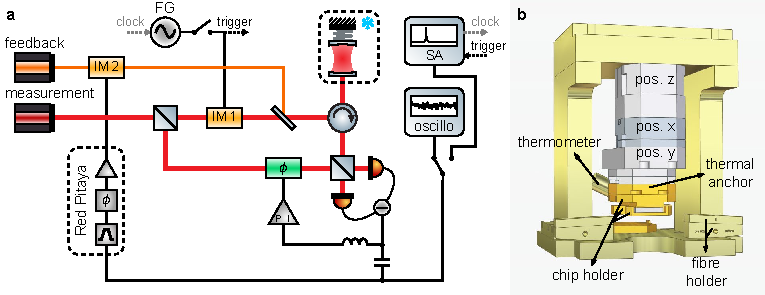
\includegraphics{methods_figs/paper_setup_v3.pdf}
    \caption{\textbf{Experimental setup. a,} Control and measurement circuitry. IM, intensity modulator (electro-optic). FG, function generator. SA, spectrum analyzer. oscillo, oscilloscope. PI, proportional--integral controller. The $\phi$-labelled green box indicates a fibre stretcher. An on-resonance laser beam (red) interacts with the optomechanical device located inside a dilution refrigerator. The mechanical displacement is imprinted on the phase quadrature of the back-reflected beam, allowing the resonator’s motion to be monitored via homodyne detection. The measurement data is recorded by the oscilloscope. To stabilise the device, weak feedback is applied using a detuned laser (orange) and IM~2. IM~1 and the SA are used only for characterisation.
    \textbf{b,} Holding structure. The chip, with the optomechanical device fabricated on top, is placed upside-down in a holder and mounted onto a stack of three piezo-positioners (pos. x, y, z) to provide three-axis motorised control. The tapered fibre is fixed into place with adjustable angle to optimise alignment. A thermal anchor is sandwiched between chip holder and positioning stack, while a thermometer provides temperature readings. The full structure is placed on the bottom of the dilution refrigerator, over a series of windows that allow optical access for alignment.
    }
    \label{fig:methods_setup}
\end{figure*}

\subsection{Efficient optical coupling}
\label{sec:methods:optical_coupling}
To attain high $\eta$, we require an efficient interface between the cavity and the fibre-based interferometer. This is provided by a short on-chip silicon nitride waveguide that evanescently couples to the cavity with high efficiency ($\eta_\text{esc} = 82$\%, section~\ref{sec:methods:char_optical}) and ends on one side in a photonic crystal mirror and, on the other, in a tapered section. 
From the waveguide taper, light is transferred adiabatically into a conically tapered single-mode fibre that is brought into contact.

Maximising waveguide--fibre transfer efficiency $\eta_\text{wf}$ requires the fibre tip to have the appropriate tapering profile. Inspired by Ref.~\cite{tiecke2015efficient}, we fabricate this using a home-built heat-and-pull setup (based on a hydrogen torch) and an off-the-shelf solenoid (RS Components 177-0146, for fast pulling) \cite{khademi2024optomechanical}. Maximising $\eta_\text{wf}$ also requires a precise positional and angular alignment. This is challenging in a dilution refrigerator: Room-temperature pre-alignment is lost to thermal contraction on cool-down, while our in-situ cold alignment is hindered by limited visual access through five layers of heat shielding.
% 
% To maximise the waveguide-fibre transfer efficiency $\effwf$, their relative alignment in both position and angle is crucial. This is hard to achieve in a dilution refrigerator: Pre-alignment when the refrigerator is still at room temperature does not survive thermal contraction during cool-down, while in-situ alignment in the cold environment---the method we use---suffers from  limited visual access through five layers of heat shielding.
To overcome this challenge, the device alignment (and mounting) is first facilitated by a custom holding structure (Extended Data FIG.~\ref{fig:methods_setup}\textbf{b}). The tapered fibre is fixed with a grooved, angle-adjustable clamp, while the chip, containing several optomechanical devices, is mounted upside-down on a gold-plated, oxygen-free copper holder attached to a three-axis cryo-compatible piezo positioner stage (Attocube ANPx or ANPz). To enhance thermalisation, a thermal anchor (Attocube ATC100) is sandwiched between holder and stage, and linked to the base plate by a copper strip. A resistive thermometer (Lake Shore) monitors holder temperature.
% A custom holding structure, shown in Extended Data Fig.~\ref{fig:methods_setup}b, facilitates device mounting and alignment. The tapered fibre is fixed in place, with an adjustable angle, by a grooved clamp. A chip containing several optomechanical devices is mounted upside-down on a sample holder that is screwed onto a three-axis cryo-compatible positioner stage, motorised with stick-slip piezo-electric actuators (Attocube ANPz and ANPx). The sample holder is made out of oxygen-free high-thermal-conductivity copper and gold plated to reduce radiative heat transfer. To improve thermalisation, a thermal anchor (Attocube ATC100) is sandwiched between sample holder and positioner stage, and connected to the holding structure's bottom plate using a flexible strip of copper. A resisitive thermometer tracks sample holder temperatur (Lake Shore Ultra-low Temperature Rox).
The cold alignment is then performed using a long-working-distance zoom microscope with a separate white-light illumination source, both sitting outside the fridge. To suppress reflections from the five refrigerator windows, both microscope and illuminating beam are slightly tilted towards the chip.
%While the waveguide itself is hard to see, the underlying trench provides a reliable alignment guide
With all these measures in place, we achieve $\effwf = 77\%$ (including losses in the 8-m cryostat fibre and splices) --- a notably high efficiency for a movable in-fridge optical fibre-chip interface.

%We employ a camera attached to a zooming microscope with a long working distance (Navitar \temp{...}) to image the device and fibre from below through five windows, one in each heat shield. A white light source outside the cryostat illuminates the chip. To reduce back-reflection at each window and increase contrast, microscope and light source are slightly angled. Although the waveguide is hard to identify, the wider trench underneath can be seen on the camera image. With this as a guide for aligning, we achieve a waveguide-fibre coupling of at least $\effwf > 76.7$\% (section~\ref{sec:methods:total_losses}). This figure includes losses in the long DR optical fibre as well, with several splicing points. \temp{Achieving such an efficient optical interface in a dilution refrigerator represents a significant challenge (achievement).}

\subsection{Vibration-reduced refrigeration}

In normal operation, the refrigerator pulse tube, providing cooling power, induces substantial vibrations that modulate waveguide–fibre coupling, optical path length, and signal-arm polarisation. We therefore run the experiment with the pulse tube off, cooling instead via a helium ``battery" mounted on the $4$-K flange: a pre-charged vessel of liquid helium whose evaporation sustains low temperature for about three hours. As the helium battery cools only the $4$-K flange and other cryostat flanges gradually heat up during the run, the probe fibre (which is mounted on all flanges) can make a polarisation change which we regularly check and compensate.

\subsection{Stabilising feedback}
\label{sec:methods:setup_feedback}
For input optical powers $P_\text{in} > 60$~nW (injected into the long fibre going to the cryostat), 
we observe intermittent instability of the optomechanical device, characterised by high-amplitude self-oscillations (Extended Data FIG.~\ref{fig:methods_eta_check}\textbf{a}). Similar behaviour has been previously reported in these ultra-coherent optomechanical resonators~\cite{guo2021bringing} and attributed to coherent feedback from stray back-reflections. Alternatively, large fluctuations could result in nonlinear cavity dynamics that induce effective amplification~\cite{aspelmeyer2014cavity}. 

A minimal amount of measurement-based feedback, which reduces amplitude and broadens linewidth, stabilises the resonator. It is implemented optically by modulating a weak, slightly red-detuned laser (Santec TSL-550). 
%input power $\Pfb = 0.5$ nW,
%adding $0.13$ detuned photons to the cavity).
We verify that
%the resulting dynamical backaction alters $\Gamma$ by at most $1$\% and
the feedback and measurement lasers beat only at frequencies larger than $1$ GHz, beyond the resonator’s response. This feedback laser is kept off during most characterisation.

The real-time electronic feedback signal is generated from the photocurrent by a digital signal processor (Red Pitaya STEMlab 125-14 LN). This processor implements two band-pass filters with tuneable gain and phase shift. One filter is centered at $\Omega/2\pi$ (with a $3$-dB bandwidth of $9.7$~kHz) and adjusted to stabilise the mechanical mode of our interest (section~\ref{sec:methods:char_feedback}). The other filter is set to cool a higher-order mode that starts to lase once the fundamental mode is under control.
The generated signal is then further amplified and used to drive an electro-optic amplitude modulator (Oclaro AM1). %\temp{after amplification (Mini-Circuits ZHL-32A+)}
%While the filter phase shift is adjusted to leave the peak of the mechanical susceptibility unchanged, the electronic gain is set to increase the mechanical decay rate to $\Gammafb/2\pi = 85$~Hz (section~\ref{sec:methods:char_feedback}).
%Moreover, another digital filter is implemented to cool a higher-order mode that starts to lase once our fundamental mode is under control.
As the dynamical range of the feedback setup is limited, it is only effective when engaged in the non-lasing state of the device. To ensure this, we monitor the photocurrent on the setup oscilloscope before turning on the feedback.

\section{Characterisation}
\label{sec:methods:characterisation}
We here explain the methods used to characterise the system. 

\subsection{Optical cavity}
\label{sec:methods:char_optical}
To characterise the optical cavity, we inject a low power ($\Pin = 20$~nW) from the measurement laser (feedback laser off), step the laser frequency $\omgL/2\pi$ across the cavity response (with resonance frequency $\omgc/2\pi$ and decay rate $\kappa$) and measure the average intensity of the back-reflected light (Extended Data FIG.~\ref{fig:methods_optical_char}\textbf{a}). Considering the field reflection ratio
\begin{equation}
    \mathcal{R}=\dfrac{(1-2\eta_\text{esc})+2 i \Delta/\kappa}{1+2 i \Delta/\kappa}
\end{equation}
with $\Delta=\omgc-\omgL$, we fit $|\mathcal{R}|^2$ to the measured intensity response and find $\omgc/2\pi = 194.898$~THz, $\kappa/2\pi = 11.50$~GHz and $(1-2\eta_\text{esc})^2=0.40$.
\begin{figure}
    \centering
    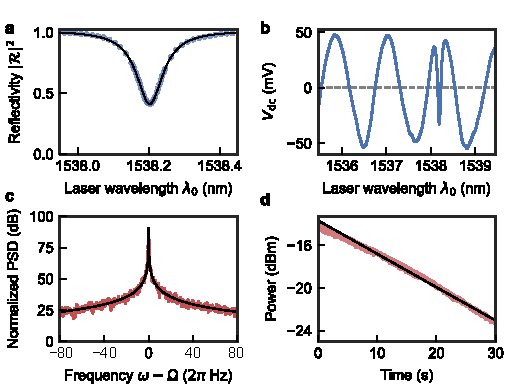
\includegraphics{methods_figs/mfig001b_ADDED_optical_mechanical_v2exp.pdf}
    \caption{\textbf{Cold optical and mechanical characterisation. a, } Cavity reflectivity $|\mathcal{R}|^2$ is measured (circles) as the drive laser wavelength $\lambda_0 = 2\pi c / \omgL$ is stepped over the optical resonance. The theoretical function (line) is fit to the measurements with linewidth $\kappa/2\pi = 11.50$~GHz. \textbf{b,} Overcoupling test. The DC output $V_\text{dc} \sim \Re[\mathcal{R}\exp{(i\omgL L/c)}]$
    of the balanced detector is measured as the laser wavelength is quickly swept
    %across the optical resonance $\omgc$,
    without locking the interferometer phase
    %$\Delta\phi = \omgL(\Delta L /c)$
    --- $L$ is the optical path difference between the two arms.
    %In this instance, $\Delta\phi \approx 0$ around $\omgL \approx \omgc$, so that we find $\Re[e^{\rmi \Delta\phi} \mathcal{R}(\omgc)] \approx \Re[\mathcal{R}(\omgc)] < 0$,
    As here $\exp{(i\omgL L/c)}\approx1$ at $\omgL=\omgc$, the negative sign of $V_\text{dc}$ at the resonance wavelength indicates that the cavity is overcoupled. 
    \textbf{c,} Mechanical spectrum around the resonance frequency $\Omega/2\pi=1.04$~MHz (with feedback off).
    \textbf{d,} Mechanical ring-down. An exponential decay is fitted with intrinsic energy decay rate $\Gamma = 2\pi\times(11.5\,$mHz).}
    \label{fig:methods_optical_char}
\end{figure}

To determine the sign in $\eta_\text{esc}=(1\pm\sqrt{0.40})/2$ (overcoupling or undercoupling of the cavity to the waveguide), we perform a test using the homodyne interferometer. While the laser wavelength is swept very quickly, across a $4$-nm interval, we record the DC output of the balanced detector (without locking on any homodyne phase). The interferometer then measures $\Re[\mathcal{R}\exp{(i\omgL L/c)}]$ where $L$ is the optical path difference between the two arms and $c$ is the speed of light in vacuum. While $L$ is almost constant during a single sweep, it has random changes each time that we do the measurement. We repeat this measurement until we find $\exp{(i\omgL L/c)} \approx 1$ at $\omgL=\omgc$, so the measurement output at this frequency approximates $\Re[\mathcal{R}]$ for $\Delta=0$. As shown in Extended Data FIG.~\ref{fig:methods_optical_char}\textbf{b}, this output is negative, indicating that the cavity is overcoupled and $\eta_\text{esc}=(1+\sqrt{0.40})/2$. In this figure, the 1.2-nm fringe spacing indicates that the optical path lengths of the two arms are different by about 2 mm.

\subsection{Mechanical resonator}
\label{sec:methods:char_mechanical}
The mechanical resonance frequency, $\Omega/2\pi = 1.04355$ MHz, is obtained by fitting the mechanical spectrum recorded with the setup spectrum analyser (Keysight EXA N9010A).
During cryostat cool-down, gas molecules condense onto the optomechanical device. To remove these, we induce a local boil-off: We repeatedly sweep the laser over the optical resonance at a slow rate ($1$~nm/s) and gradually increase the injected power. When $\Pin \approx 9~\mu$W, the cavity resonance swiftly shifts to a shorter wavelength by $0.5$~nm, indicating loss of dielectric material. We also find that $\Omega/2\pi$ has shifted up by about 600~Hz, indicating a loss of mass commensurate.

% \begin{figure}
%     \centering
%     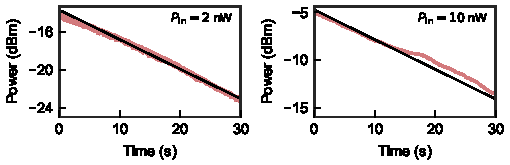
\includegraphics[width=\linewidth]{methods_figs/mfig002_resonator_ringdown.pdf}
    
%     \label{fig:methods_ringdown}
% \end{figure}

The mechanical decay rate $\Gamma$ is determined by a ring-down measurement, where the intensity of the measurement laser (with $\Pin = 2$~nW) is weakly modulated at frequency $\Omega/2\pi$ using an electro-optic modulator (Oclaro AM1) for $0.2$~s, after which the mechanical signal is recorded for $30$~s using the spectrum analyser's zero-span function (Extended Data FIG.~\ref{fig:methods_optical_char}\textbf{d}).
Fitting an exponential decay function yields $\Gamma/2\pi=11.5$~mHz. The modulation tone is produced by a signal generator (Siglent SDG) that also triggers acquisition and is referenced to the spectrum analyser's clock.

%at cryogenic temperatures (quality factor $\mathcal{Q}=9.1 \times 10^7$).



% Boil-off, mechanical resonance frequency, ringdowns.

\subsection{Optomechanical coupling}
\label{sec:methods:char_coupling}
We evaluate the single-photon optomechanical coupling rate $g_0$ from the optical spring effect \cite{bowen2015quantum}, by sweeping the laser wavelength over the cavity response and recording the mechanical spectra.

At constant, very low injected power $\Pin = 2$~nW (Extended Data FIG.~\ref{fig:methods_spring_shift}a), we find that the effective resonance frequency $\Omega_\text{eff}$ closely follows the cavity photon number $\bar{n}_\text{cav}$ and the asymmetry around $\Delta=0$, typical to the spring effect, is almost absent. We consider this as a static photothermal effect corresponding to the expected rise in the device temperature by optical absorption (from 3.5 K towards 12.1 K, section~\ref{sec:methods:mode_temperature}) --- a similar shift has been reported by Refs.~\cite{usami2012optical,hauer2019dueling}. In Extended Data FIG.~\ref{fig:methods_spring_shift}\textbf{d}, $\Omega_\text{eff}$ is shown as a function of $\bar{n}_\text{cav}$ when $\Delta = 0$. While it sharply increases at small values of $\bar{n}_\text{cav}$, the thermal shift saturates after $\nc \approx 7$. Repeating this measurement with $\Pin = 60$~nW (Extended Data FIG.~\ref{fig:methods_spring_shift}\textbf{b}), we find a distinct $\Delta$-asymmetric optical spring on top of the $\Delta$-symmetric thermal shift.
\begin{figure*}
    \centering
    % 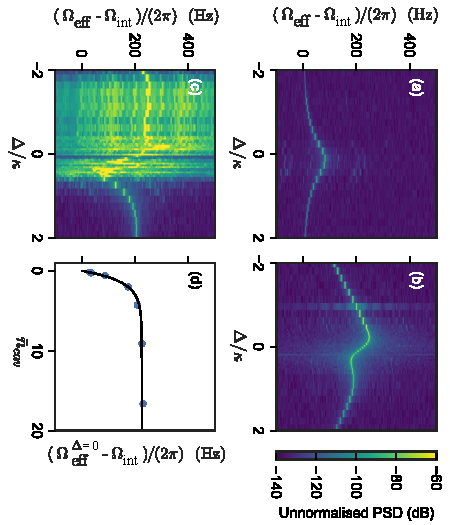
\includegraphics[width=0.49\linewidth]{methods_figs/mech_shifts_constant_power.pdf}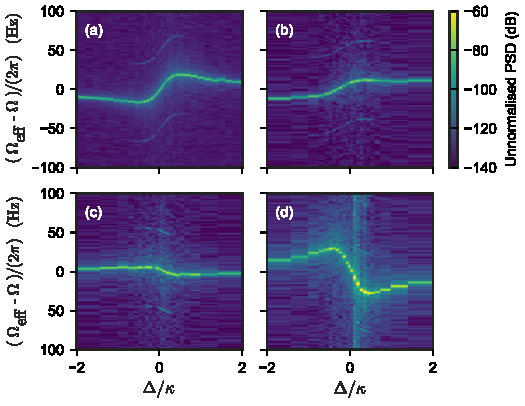
\includegraphics[width=0.49\linewidth]{methods_figs/mech_shifts_constant_nc.pdf}
    % 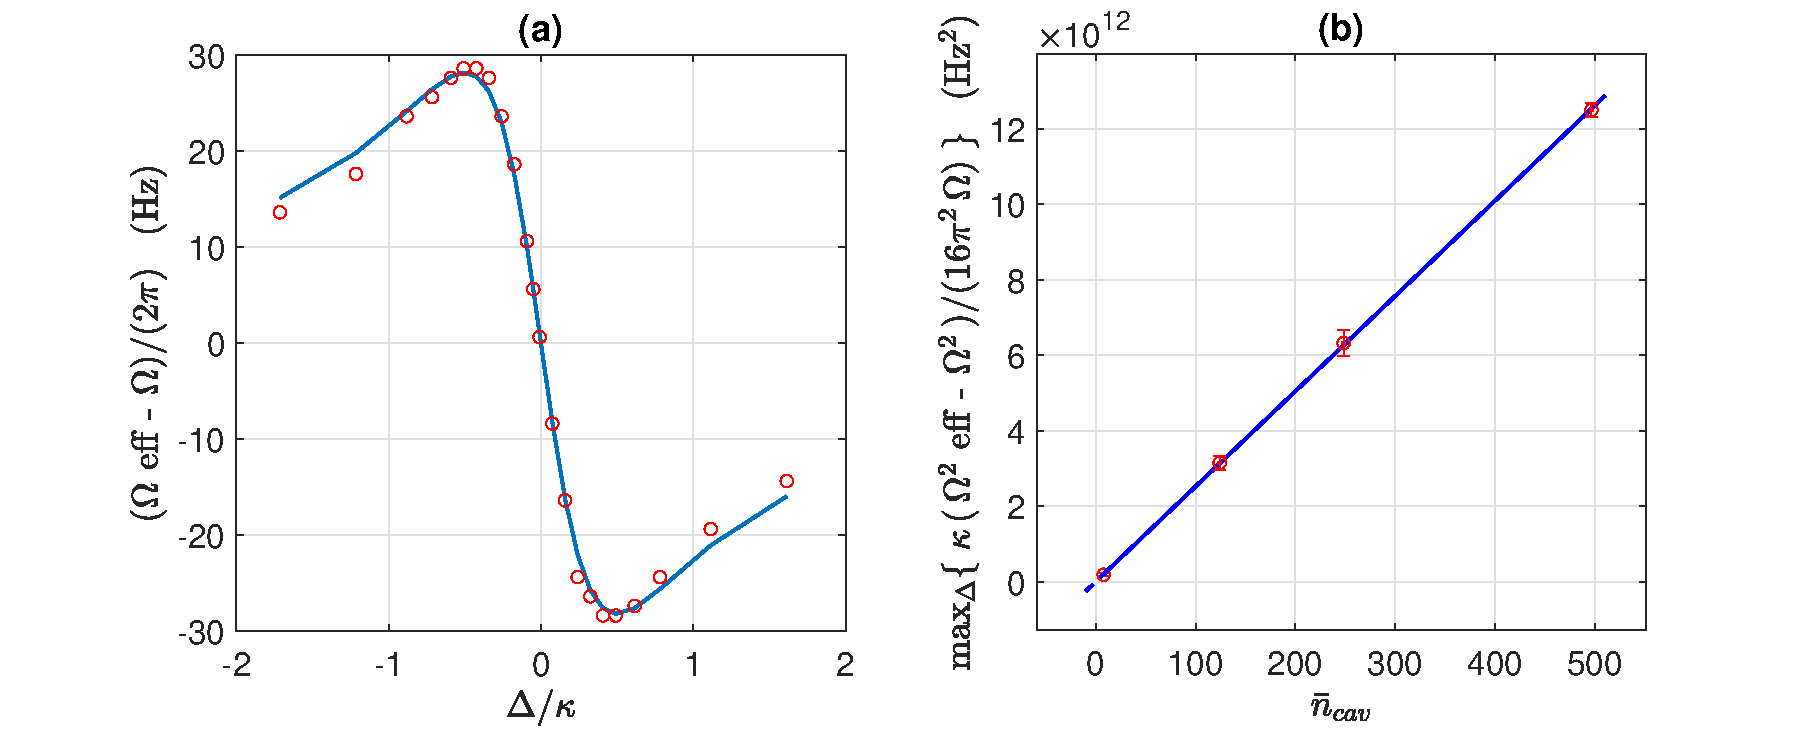
\includegraphics[width=0.49\linewidth]{methods_figs/Spring.pdf}
    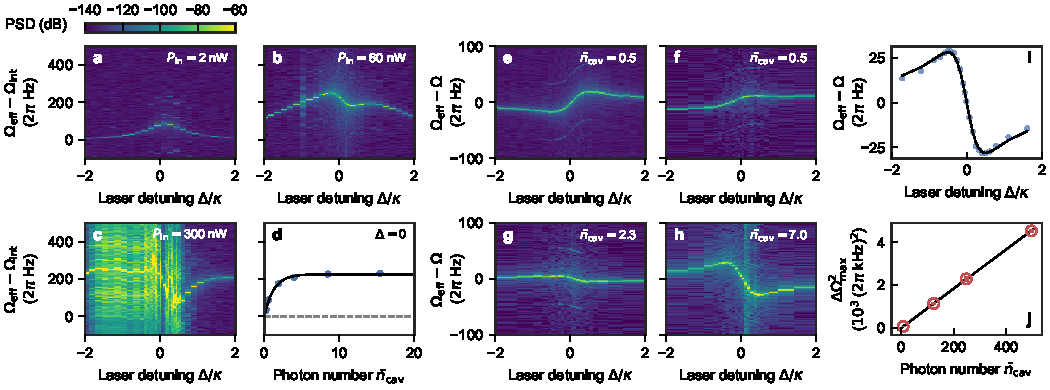
\includegraphics{methods_figs/mfig003_optomech_spring_shifts.pdf}
    \caption{\textbf{Cold characterisation of single-photon optomechanical coupling rate. a-c,} Mechanical spectra of the fundamental mode ($\Omega_\text{int}$) as the laser detuning $\Delta$ is varied, with constant input power $P_\text{in}$ and feedback laser off. For low power $P_\text{in}=2$~nW (\textbf{a}), the typical detuning-asymmetric spring shift behaviour is absent. Instead, the mechanical frequency $\Omega_\text{eff}$ tracks the cavity photon number $\bar{n}_\text{cav}$, indicating an absorption-induced thermal shift. For intermediate power $P_\text{in}=60$~nW (\textbf{b}), the optical spring effect appears on top of the thermal shift. For higher power $P_\text{in}=300$~nW (\textbf{c}), high-amplitude self-oscillations occur at both positive and negative detunings. \textbf{d,} Mechanical resonance frequencies $\Omega_\text{eff}$ extracted from mechanical spectra measured on resonance ($\Delta = 0$) for a range of photon numbers $\bar{n}_\text{cav}$. A thermal shift is observed at lower cavity intensities that saturates once $\nc\gtrsim7$. An exponential saturation curve is fitted for reference. \textbf{e-h,} Mechanical spring shift spectra for constant cavity photon number $\bar{n}_\text{cav}$, measured around the thermally shifted mechanical frequency $\Omega$ with feedback laser off. At the lowest $\bar{n}_\text{cav} = 0.5$, an inverted spring shift stemming from photothermal back-action is observed. The shift is stronger before condensed gas boil-off (\textbf{e}) than after (\textbf{f}). At intermediate $\bar{n}_\text{cav} = 2.3$ (\textbf{g}), radiation pressure and photothermal back-action tend to cancel each other, leading to a small spring effect. At a higher $\bar{n}_\text{cav} = 7.0$ (\textbf{h}), where the thermal shift in panel \textbf{d} is saturated, a strong optical spring with the typical
    detuning dependence is observed. \textbf{i,} Radiation-pressure-induced spring is fitted to the mechanical frequencies extracted from panel \textbf{h}. \textbf{j,} Maximal squared spring shift $\Delta \Omega_\text{max}^2 = \max_\Delta\{|\Omega_\text{eff}^2 - \Omega^2|\}$ obtained from measuring at the three detunings $\Delta = 0, \pm \kappa/2$ with high values of $\nc$. Error bars represent the difference between the measured values of $\Delta \Omega_\text{max}^2$ with $\Delta = +\kappa/2$ and $\Delta = -\kappa/2$, while the data points are found by averaging those values. For radiation-pressure-induced spring, $\Delta \Omega_\text{max}^2=4\Omega g_0^2/\kappa\times\nc$. The reliable linear fit (with a zero y-intercept) gives the single-photon coupling rate as $g_0/2\pi=159$~kHz.}
    \label{fig:methods_spring_shift}
\end{figure*}

To isolate the optical spring effect, we do the measurement by keeping $\nc$ (and thus the thermal shift) constant across the sweep interval --- $\Pin$ is changed at each value of $\Delta$. For low $\nc = 0.5$ (Extended Data FIGs.~\ref{fig:methods_spring_shift}\textbf{e} and~\textbf{f}), we find an optical spring effect with detuning dependence opposite to a radiation-pressure-induced spring. That is, we find higher $\Omega_\text{eff}$ at $\Delta > 0$ than at $\Delta < 0$. We attribute this to the dynamical backaction of a dominating deformation force opposing the radiation pressure. This force is considered to be caused by a temperature gradient profile across the solid structure made by local absorption heating and the poor thermal conductivity of silicon nitride at low temperatures, similar to what has been reported by Ref.~\cite{hauer2019dueling}. Interestingly, this effect is stronger before the condensed gas molecules are boiled off (Extended Data FIG.~\ref{fig:methods_spring_shift}\textbf{e}), possibly indicating higher local absorption.

For a moderate $\nc = 2.3$ (Extended Data FIG.~\ref{fig:methods_spring_shift}\textbf{g}), we see the net spring effect switches sign. This is to be expected: By the rise of the device temperature, there should be a sharp increase in the thermal conductivity --- see, e.g., Ref.~\cite{ftouni2015thermal} --- suppressing the photothermal force and allowing the radiation pressure to dominate, similar to what has been reported by Ref.~\cite{hauer2019dueling}. With further increase of $\nc$ to 7, near the saturation limit in Extended Data FIG.~\ref{fig:methods_spring_shift}\textbf{d}, we find a strong optical spring with the typical detuning dependence (Extended Data FIG.~\ref{fig:methods_spring_shift}\textbf{h}). Fitting the radiation-pressure-induced spring~\cite{bowen2015quantum} on this data (Extended Data FIG.~\ref{fig:methods_spring_shift}\textbf{i}) gives a value of $155$~kHz for $g_0/2\pi$.

The photothermal force is then expected to be negligible for $\nc\gtrsim7$, leaving the spring effect solely driven by radiation pressure (with maximum values for $|\Omega_\text{eff}^2-\Omega^2|$ scaling linearly with $\nc$, as $g_0$ is independent of $\nc$). To verify this expectation, we need to do the measurement for higher $\nc$ where we encounter intermittent instability of the system (Extended Data FIG.~\ref{fig:methods_eta_check}\textbf{a}) and have to adapt our technique. We reduce the laser sweep to the three detunings $\Delta = 0, \pm\kappa/2$ where the spring shift (with constant $\nc$) is zero or maximal. At each detuning, we monitor the system on the oscilloscope and once it is in the non-lasing state, we record a 1-s time trace. Calculating the spectrum of the recorded trace, we extract the value of $\Omega_\text{eff}$. Performing this adapted measurement with multiple high values of $\nc$ strongly confirms the linear scaling (Extended Data FIG.~\ref{fig:methods_spring_shift}\textbf{j}) and characterises the coherent single-photon coupling rate as $g_0/2\pi=159$~kHz.

\subsection{Feedback loop}
\label{sec:methods:char_feedback}
%To optimize the phase $\arg[\Hfb(\Omega)] \approx \pi/2$ of the feedback filter transfer function $\Hfb(\omega) \propto \grp$, we engage the feedback system with a low electronic gain setting $\grp$ on the Red Pitaya and tune the electronic phase shift $\phirp$, until we can broaden the mechanical linewidth without changing the resonance frequency (both extracted by fitting thermomechanical spectra). 
The performance of the feedback loop is characterised and optimised by sweeping the electronic gain setting $\grp$ on the Red Pitaya and taking mechanical spectra (Extended Data FIG.~\ref{fig:methods_feedback}\textbf{a}), while the measurement and feedback laser power are the same as the final collection of monitoring data ($\Pin=154.0$~nW and $\Pfb = 0.5$~nW, respectively). By fitting on these mechanical spectra, we extract the feedback-broadened linewidth $\Gammafb$, the resonance frequency and the peak area as functions of $\grp$.
%\begin{align}
%    S_{YY}(\omega) &= 1 + 16 \eta \frac{g_0^2 \nc}{\kappa}  \frac{\Gammafb}{(\omega-\Omega)^2 + \Gammafb^2/4} \times \bar{n} \label{eq:methods:Syy_feedback}
    % \\ &= 1+4\eta \Cfb \frac{\Gammafb^2}{(\omega-\Omega)^2 + \Gammafb^2/4} \times \bar{n} \nonumber
%\end{align}
%where $S_{YY}(\omega)$ is normalised to optical measurement shot noise%
% and $\Cfb = 4 g_0^2 \nc / (\kappa \Gammafb)$
We verify that $\Gammafb$ scales linearly with $\grp$ (Extended Data FIG.~\ref{fig:methods_feedback}\textbf{b}, left), while the resonance frequency does not change (same figure, middle). This optimised performance is achieved by tuning the electronic phase shift setting on the Red Pitaya (such that $\arg[\Hfb(\Omega)] \approx \pi/2$, where $\Hfb(\omega) \propto \grp$ is the feedback loop transfer function). Importantly, we also verify that the peak area scales with $1/\Gammafb$ (Extended Data FIG.~\ref{fig:methods_feedback}\textbf{b}, right), indicating that we are not feeding excess noise onto the resonator.
\begin{figure}
    \centering
    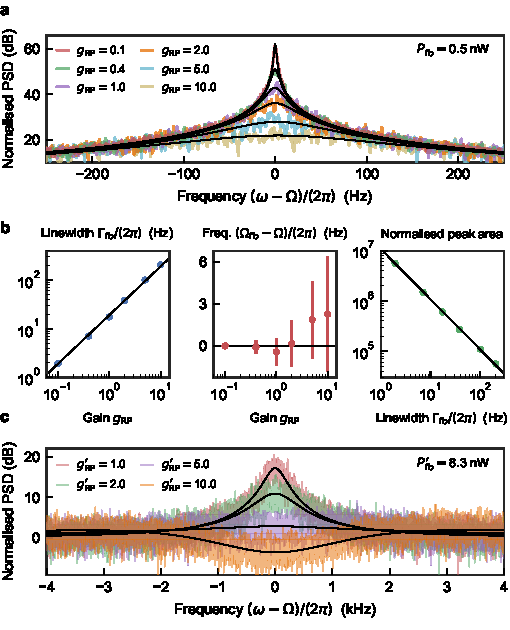
\includegraphics{methods_figs/mfig004_feedback.pdf}
    \caption{\textbf{Feedback loop performance. a,} Mechanical spectra, normalised to the shot noise level, for increasing feedback voltage gain $g_\text{RP}$ at low feedback laser power $P_\text{fb} = 0.5$~nW. A Lorentzian function
    %Eq.~\eqref{eq:methods:Syy_feedback}
    is fitted (lines) with increasing linewidth and decreasing height. \textbf{b,} Estimated linewidths $\Gamma_\text{fb}$, frequencies $\Omega_\text{fb}$ and peak areas from panel \textbf{a}. A linear fit is shown for $\Gamma_\text{fb}$ versus $g_\text{fb}$, while a reciprocal fit is plotted for area versus $\Gamma_\text{fb}$. The error bars in the middle plot indicate the fit errors. \textbf{c,} Mechanical spectra for higher feedback laser power $\Pfb' = 8.3$~nW. With a strong feedback gain, noise squashing is observed.}
    \label{fig:methods_feedback}
\end{figure}

To evaluate how far we are from the noise squashing regime, where there is a significant correlation between the measurement noise and the resonator process noises, we repeat this experiment with more feedback laser power $\Pfb' = 8.3$~nW. As shown in Extended Data FIG.~\ref{fig:methods_feedback}\textbf{c}, we observe noise squashing once $\grp' > 7$, equivalent to $\grp \approx \grp' \Pfb' / \Pfb > 116$ (at the main feedback power).

%We also use a network analyser to measure the extra delay of the feedback loop. It is about 1~$\mu$s.
The gain that we choose for the final collection of monitoring data is then $\grp = 4$, well below the squashing limit, resulting in $\Gammafb/2\pi = 85$~Hz. We note that with $\nc=41.4$ measurement photons (provided by the $\Pin=154$~nW input power), the average number of detuned feedback photons in the cavity is only 0.13, making the consequent dynamical backactions and excess optical noise negligible.

\subsection{Resonator temperature}
\label{sec:methods:mode_temperature}
An accurate estimate of the mechanical resonator’s effective temperature is crucial for our analysis. However, because of its long intrinsic decay time, $1/\Gamma \approx 14$~s, sampling the full thermal amplitude distribution takes a long time. We assess that achieving a 10\% relative accuracy in the estimated mean energy would require monitoring the resonator in the non-lasing state for about an hour, which is impractical as the system is unstable.

We therefore estimate the average energy with the feedback on, as the system is stable and $1/\Gammafb$ is much shorter than $1/\Gamma$. In particular, we extrapolate the reciprocal fit shown in Extended Data FIG.~\ref{fig:methods_feedback}\textbf{b}, right, to find the total phonon number $n_\text{tot} = \mathcal{C} + \nth + 1/2$ at the intrinsic linewidth ($\Gammafb = \Gamma$, where $\grp = 0$). After subtracting $\mathcal{C} + 1/2$, we are left with a value for $\nth$ that corresponds to the temperature $T = 12.1$~K. This is significantly higher than the fridge temperature (3.5~K), consistent with our expectation in section~\ref{sec:methods:char_coupling}.

Considering the characterised values of $T$ and $g_0$, the ratio $\mathcal{C}/n_\text{th}$ with $\bar{n}_\text{c}=41.4$ is large enough to produce a measurable level of ponderomotive squeezing of light. We verify this by changing the lock point of our homodyne setup from the phase quadrature $(\phi=90\degree)$ to $\phi=130\degree$ and recording the mechanical spectrum. We note that, with the feedback power unchanged ($\Pfb=0.5$~nW) and the Red Pitaya gain set at $g_\text{fb}^\phi=1$, the feedback-induced correlation of the measurement noise and the process noises is negligible --- the effective gain $g_\text{fb}=\sin{(\phi)}\times g_\text{fb}^\phi\approx0.77$ is more than two orders of magnitude lower than the squashing limit. The recorded spectrum (Extended Data FIG.~\ref{fig:methods_pond_sqz}) shows ponderomotive squeezing and the corresponding asymmetry around $\Omega$, confirming the considerable ratio of backaction heating to thermal heating.
\begin{figure}[t!]
    \centering
    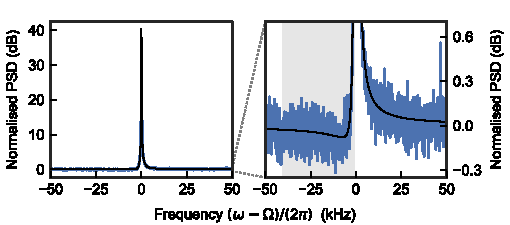
\includegraphics{methods_figs/mfig005e_ponderomotive_squeezing.pdf}
    \caption{\textbf{Ponderomotive squeezing.} Photocurrent spectral density (in dB, collected with a 100-Hz resolution bandwidth, normalised to the shot noise level) measured with the homodyne interferometer tuned to an intermediate optical quadrature ($\phi = 130\degree$). Optical correlations mediated by the mechanical resonator give rise to ponderomotive squeezing (negative values) and render the spectrum highly asymmetric around $\Omega$. Fitting Eq.~\eqref{eq:methods:Syy_ponderomotive} to the grey-shaded region yields estimates of the single-photon optomechanical coupling $g_0$ and the resonator temperature $T$.}
    \label{fig:methods_pond_sqz}
\end{figure}

We also use this demonstration of ponderomotive squeezing to double-check the values of $g_0$ and $T$. This is possible because the recorded spectrum (once normalised to the shot noise level) approximates
\begin{align}
\begin{aligned}
    S(\omega) = &1 + 16\eta\,|\Gamma\chi(\omega)|^2  \sin^2(\phi) \times \mathcal{C}\,n_\text{tot} \\
    &+ 4 \eta\,\Re[\Gamma\chi(\omega)] \sin(2\phi)\times  \mathcal{C}
\end{aligned} \label{eq:methods:Syy_ponderomotive}
\end{align}
(with $\chi(\omega)=\Omega/(\Omega^2-\omega^2-i\omega\Gamma)$ and all the feedback replacements $\Gamma\rightarrow\Gamma_\text{fb}$ and $\nth\rightarrow\nth\times\Gamma/\Gamma_\text{fb}$ in place), where the squeezing term (the last one on the right hand side) is independent of $\nth$. By fitting Eq.~\ref{eq:methods:Syy_ponderomotive} (Extended Data FIG.~\ref{fig:methods_pond_sqz}), we get 160.59~kHz for $g_0/2\pi$ and 12.19~K for $T$, in good agreement with previous results.

%From the optical fluctuation spectrum Eq.~\eqref{eq:methods:Syy_feedback}, which applies when the phase difference $\theta = \pi/2$ of the homodyne detector is tuned to measure the phase quadrature, $g_0$ and $\bar{n}$ cannot be fitted independently. Ponderomotive squeezing of the light, where optical correlations are mediated by the mechanical resonator~\cite{bowen2015quantum}, can be observed when moving $\theta$ off the phase quadrature. For general $\theta$, the optical spectrum reads ... with susceptibility $\chi(\omega) = -1/(\rmi \Gamma + 2\Delta)$. The last term describes ponderomotive squeezing and can be negative. Moreover, it is independent of $\bar{n}$, so that fitting Eq.~\eqref{eq:methods:Syy_ponderomotive} gives independent estimates of $g_0$ and $\bar{n}$.


%As a sanity check, we estimate $g_0$ and $\bar{n}$ from ponderomotive squeezing. We set $\theta = 130\degree$, apply weak feedback with $\grp^\theta = 1$, and record a thermomechanical spectrum (Extended Data Fig.~\ref{fig:methods_pond_sqz}). As rotating $\theta$ reduces the homodyne detector's sensitivity to mechanical displacement, $\grp^\theta=1$ is equivalent to $\grp = \sin(130\degree) \grp^\theta = 0.77$ at $\theta = \pi/2$. This is more than two orders of magnitude below the squashing limit, such that optical correlations introduced by the feedback are negligible. We thus fit Eq.~\eqref{eq:methods:Syy_ponderomotive} to the data after replacing $\Gamma \to \Gammafb$, $\mathcal{C} \to \Cfb$, and find estimated values $g_0/(2\pi) = 160.6$~kHz and $T=12.2$~K, in good agreement with previous results.

\subsection{Optical detection efficiency}
\label{sec:methods:total_losses}
In Extended Data TABLE~\ref{tab:methods:efficiency}, we quantify the various inefficiencies encountered by the probe field on its way from the optical cavity to the final phase detection.
%Combining these, we find the total detection efficiency $\eta = 37.9\%$. All input powers $\Pin$ and $\Pfb$ listed for the main and feedback lasers, respectively, are measured right before entering the long cryostat fibre. To relate these to the cavity photon number $\nc$, we use $\effc$ and $\effwf$.
\begin{table}[]
    \centering
    \begin{tabular}{l|c}
        efficiency element & value \\
        \hline
        cavity--waveguide coupling ($\eta_\text{esc}$) & $81.8\%$ \\
        waveguide--fibre coupling ($\effwf$, in the dilution fridge) & $76.7\%$ \\
        interferometer components' transmission & $83.2\%$ \\
        interference visibility & $99\%$ \\
        photodetector quantum efficiency & $76\%$ \\
        electronic noise suppression & $96.7\%$ \\
        \hline
        total efficiency ($\eta$) & $38\%$
    \end{tabular}
    \caption{\textbf{Contributions to optical detection inefficiency.}}
    \label{tab:methods:efficiency}
\end{table}

\subsection{Estimating optical detection efficiency from non-linear transduction}
\label{sec:methods:eta_check}
To obtain an independent estimate of the total efficiency $\eta$, we developed a new method based on the nonlinear transduction of high-amplitude mechanical motion by the optical cavity~\cite{leijssen2017nonlinear}. In our experiment, we can readily access this regime by turning the feedback off and waiting for instability to occur. Extended Data FIG.~\ref{fig:methods_eta_check}\textbf{c} shows a time trace of a photocurrent obtained under such conditions.

In this method, we use the extreme values of the phase quadrature component of the reflectivity $\Im[\mathcal{R}] = \effc \kappa \Delta/(\Delta^2 + \kappa^2/4)$ (Extended Data FIG.~\ref{fig:methods_eta_check}\textbf{b}) as a reference level. These extrema are located at $\Delta = \pm \kappa/2$, where $\Im[\mathcal{R}] = \pm \effc$, and occur in Extended Data FIG.~\ref{fig:methods_eta_check}\textbf{c} as the mechanically-shifted instantaneous detuning $\Delta = g_0 Q$ explores a large fraction of the cavity response. Here, $Q$ is the mechanical displacement normalized to its zero point fluctuations.
\begin{figure}
    \centering
    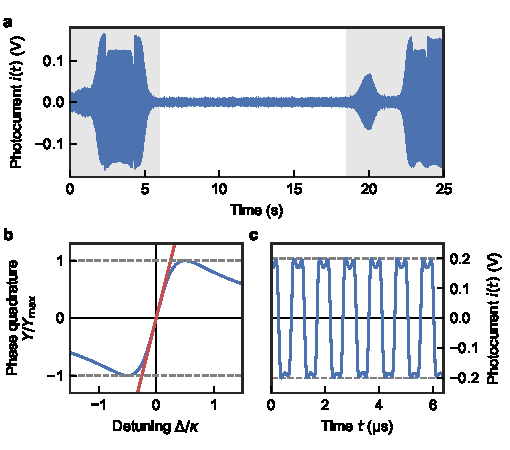
\includegraphics{methods_figs/mfig006_eta_check.pdf}
    \caption{\textbf{Non-linear transduction of high-amplitude oscillations. a,} Intervals of intermittent instability (grey) in the mechanical amplitude are observed for higher input powers, when the feedback laser is off. These intervals get longer and more frequent with increasing laser power. \textbf{b,} Phase quadrature $Y$ of the mean intra-cavity field as a function of detuning $\Delta$ (blue). Extreme values $\pm Y_\text{max}$ are indicated (dashed lines) and occur at $\Delta = \pm \kappa/2$. For small detunings $|\Delta| \ll \kappa$, the linear approximation (red) is typically used. \textbf{c,} High-amplitude self-oscillations of the resonator explore detunings beyond $|\Delta| > \kappa/2$. The extreme values in the photocurrent (dashed lines) then correspond to $\pm Y_\text{max}$ and can be used for calibration.}
    \label{fig:methods_eta_check}
\end{figure}

We proceed by switching to a semi-classical picture and writing the detected phase quadrature as
\begin{align}
    \Ydet = \Yv + \sqrt{\eta \kappa} Y \label{eq:methods:Ydet_1}\,,
\end{align}
the sum of a quantum vacuum field $\Yv$ and a classical field, where
\begin{align}
    Y = 2 \sqrt{\effc \kappa}\,\Im[\chi_a]\times\alpha_\text{in} \label{eq:methods:Ycav_1}
\end{align} 
is the mean phase quadrature of the driven intra-cavity field. Here, we consider the cavity susceptibility $\chi_a = (\kappa/2 - i \Delta)^{-1}$ and the coherent amplitude~$\alpha_\text{in}$ of the field coupling in (from the waveguide, with efficiency~$\effc$). We take $\alpha_\text{in}$ real.

% Plugging Eq.~\eqref{eq:methods:Ycav_1} into Eq.~\eqref{eq:methods:Ydet_1}, we get
% \begin{align}
% \begin{aligned}
%     \Ydet &= \Yv + \sqrt{2\eta} \Im[\kappa \chi_a(\Delta)] \sqrt{\effc} \alpha_\text{in} \\
%     &= \Yv + \sqrt{2\eta} \Im[\mathcal{R}_\rmi(\Delta)]
% \end{aligned}
% \end{align}

Next, we express $\alpha_\text{in} = \sqrt{\nc\kappa/(4\effc)}$ in terms of the cavity photon number $\nc$ attained on resonance ($\Delta = 0$), and get
\begin{align}
    Y = \sqrt{\nc}\times\Im[\kappa \chi_a] = \sqrt{\nc}\times\frac{\kappa\Delta}{\Delta^2 + \kappa^2/4}\,,
\end{align}
where we note that $\Im[\kappa \chi_a] = \Im[\mathcal{R}]/\effc$.
As the instantaneous $\Delta$ is swept across the cavity resonance by mechanical motion, $Y$ attains a maximum value of $Y_\text{max} = \sqrt{\nc}$ at $\Delta = \kappa/2$, and $-Y_\text{max}$ at $\Delta = - \kappa/2$.

The homodyne detector produces a photocurrent $\rmi = s \Ydet$ proportional to the detected phase quadrature. The maximum photocurrent $\rmi_\text{max}$, as shown in Extended Data FIG.~\ref{fig:methods_eta_check}\textbf{c}, is obtained when $Y = Y_\text{max}$ and given by
\begin{align}
    \rmi_\text{max} = s \sqrt{\eta\kappa}\,Y_\text{max} = s \sqrt{\eta\kappa\,\nc}\,.
\end{align}
If $\eta$, $\kappa$ and $\nc$ are all known, we can use $Y_\text{max}$ as a reference to find the detector sensitivity $s = \rmi_\text{max} / \sqrt{\eta \kappa \nc}$.

If, however, $\eta$ is not known, we can determine it by comparing $\rmi_\text{max}$ to the shot-noise spectral density $S_{\rmi\rmi}^\text{SN}(\omega)$ of the photocurrent measured when the cavity is not driven, i.e., when $Y=0$ and $\Ydet = \Yv$. We then find
\begin{align}
    S_{\rmi\rmi}^\text{SN}(\omega) = s^2 S_{\Yv\Yv}(\omega) = \frac{\rmi_\text{max}^2}{\eta \kappa\,\nc} \label{eq:methods:eta_from_SN}
\end{align}
where $S_{\Yv\Yv}(\omega) = 1$ for the optical vacuum field $\Yv$.
To work out $\eta$ from Eq.~\eqref{eq:methods:eta_from_SN}, $\kappa$ needs to be entered as an angular frequency and $S_{\rmi\rmi}^\text{SN}(\omega)$ calculated as a double-sided spectrum. Note that to determine $\nc$, we still use $\effc$ and $\effwf$, which can be estimated independently and accurately.

In our experiment, we find $\rmi_\text{max} = 0.200$~V for $\nc = 41.4$, and a noise spectral density $S_{\rmi\rmi}^\text{SN}(\omega) = 3.53 \times 10^{-14}\  \mathrm{V}^2/\mathrm{Hz}$ around the mechanical resonance $\Omega$. Hence, from Eq.~\eqref{eq:methods:eta_from_SN} we find a value of 37.8\% for $\eta$, in good agreement with the previous result.

\section{Data acquisition and analysis}
Time traces of the photocurrent are recorded on a low-noise oscilloscope (Tektronix MSO64). The oscilloscope produces digital samples at a rate of 5 MHz with $12$-bit vertical resolution (acquisition mode Sample). The oscilloscope's maximum record length is $6.25\times10^7$~samples. To prevent aliasing, an analogue filter is placed before the oscilloscope input.

\ifSubfilesClassLoaded{% then branch
    % commands executed only if this file is compiled by itself
    \bibliographystyle{apsrev4-2}
    \bibliography{sn-bibliography}% common bib file
}{% else branch
    % commands executed only if compiled from the main file
}

\end{document}
